\documentclass[conference]{IEEEtran}
\IEEEoverridecommandlockouts

\usepackage{cite}
\usepackage{amsmath,amssymb,amsfonts}
\usepackage{algorithmic}
\usepackage{graphicx}
\usepackage{textcomp}
\usepackage{xcolor}
\usepackage{hyperref}
\usepackage{booktabs}
\usepackage{array}
\usepackage{tabularx}
\usepackage{microtype}
\usepackage{url}
\usepackage{tikz}
\usepackage{pgfplots}
\usepgfplotslibrary{polar}
\pgfplotsset{compat=1.18}
\usetikzlibrary{shapes.geometric, shapes.misc, arrows.meta, positioning,
                fit, backgrounds, shadows.blur, calc, shapes.symbols}
\newcolumntype{Y}{>{\raggedright\arraybackslash}X}
\newcommand{\tabletight}{\footnotesize\setlength{\tabcolsep}{3.5pt}\renewcommand{\arraystretch}{1.08}}

\def\BibTeX{{\rm B\kern-.05em{\sc i\kern-.025em b}\kern-.08em
    T\kern-.1667em\lower.7ex\hbox{E}\kern-.125emX}}

\begin{document}

\title{Personal Digital Data Analysis for Behavioral Insights\\
{\large CSE 458 -- Big Data Analytics -- Final Report}}

\author{
    \IEEEauthorblockN{Soner G\"{U}NE\c{S}, Mehmet Alp ATAY, Emre \.{I}lhan \c{S}ENEL, H. Muhammet \c{C}ENGEL\c{C}\.{I}}
    \IEEEauthorblockA{Department of Computer Science and Engineering\\
    CSE 458 -- Big Data Analytics}
}

\maketitle

\begin{abstract}
Music streaming platforms generate massive fine-grained event logs that
remain opaque to end users despite containing rich behavioral signals.
\textit{Datatify} is a big data analytics platform that ingests a user's
Spotify Extended Streaming History export and produces an interactive
behavioral dashboard through a three-tier distributed processing pipeline.
\textbf{Problem:} Raw streaming logs contain up to 500\,K event records
per user but existing tools expose only coarse yearly summaries; no
end-to-end open platform derives multi-dimensional behavioral profiles,
graph-theoretic listening models, and cross-user clustering from these logs.
\textbf{Method:} We implement three parallel pipeline tiers—pure-Python
$O(N)$ single-pass aggregation, Pandas vectorized groupBy, and Apache
PySpark distributed DataFrames—computing 15 behavioral metrics, a
weighted directed artist-transition graph with PageRank and
label-propagation community detection, K-Means listener clustering with
automatic optimal-$k$ selection via silhouette scoring, and an optional
Google Gemini character narrative.
\textbf{Key Results:} The pure-Python tier achieves 132\,K records/s
throughput with a median request latency of 0.38\,s on a 50\,K-record
upload. Pandas is 19.3\% faster at 2\,M records. PySpark incurs a
constant 8\,s JVM overhead, with estimated crossover at $N^* \approx
540\,000$ records. K-Means clustering reaches a silhouette score of up
to 0.61. The system passes 70 automated tests with 100\% pass rate.
\end{abstract}

\begin{IEEEkeywords}
big data analytics, distributed computing, Apache Spark, PySpark,
music streaming, behavioral profiling, artist transition graph,
listener clustering, K-Means, PageRank, community detection, FastAPI,
generative AI, personality archetypes, scalability benchmark
\end{IEEEkeywords}

% ─────────────────────────────────────────────────────────────────────────────
\section{Introduction}

\subsection{Big Data Context}

Spotify serves over 600 million active users, each generating a continuous
stream of fine-grained listening events. A single user's \emph{Extended
Streaming History}—obtainable via Spotify's privacy portal—can contain
between 50\,000 and 500\,000 records spanning multiple years, with each
record encoding timestamp, milliseconds played, track and artist metadata,
skip and shuffle flags, platform identifier, country code, and playback
start/end reasons. At population scale, these event streams constitute a
classic \emph{big data} problem: high volume (hundreds of millions of events
per day across all users), high velocity (near-real-time event generation),
and high variety (heterogeneous JSON structures with optional fields and
inconsistent platform strings).

Even at single-user scale, the analysis involves non-trivial data engineering
challenges: computing multi-dimensional aggregations over time-series event
logs, detecting session boundaries from irregular inter-arrival times,
correcting UTC timestamps for geographic timezone offsets without losing
precision, and building graph structures over millions of consecutive-play
pairs. At multi-user scale—necessary for comparative clustering—these
challenges motivate evaluation of distributed computing frameworks such as
Apache Spark.

Despite this richness, the user-facing Spotify application surfaces only
coarse summaries such as ``Spotify Wrapped,'' a once-a-year retrospective
limited to top artists and total hours. The per-event resolution in the
Extended Streaming History export enables far deeper behavioral
characterization: session topology, circadian listening rhythms, habit-loop
detection, genre-traversal patterns expressed as graph transitions, and
cross-user comparative clustering.

\subsection{Contributions}

We design and implement \textit{Datatify}, a platform that bridges the gap
between raw event logs and actionable behavioral insight. The primary
contributions of this work are:
\begin{enumerate}
  \item \textbf{A three-tier big data processing pipeline} comparing
        pure-Python, Pandas, and Apache PySpark implementations on the same
        analytical tasks, with a scalability benchmark over 100\,K–2\,M
        synthetic records establishing the crossover point at which
        distributed overhead pays off.
  \item \textbf{A 15-dimensional behavioral metric framework} derived from
        a single $O(N)$ pass over raw streaming logs, covering exploration
        breadth, loyalty depth, temporal patterns, habit formation, and
        platform usage.
  \item \textbf{A graph-theoretic listening model} representing the user's
        artist-transition behavior as a weighted directed graph with PageRank
        centrality, label-propagation community detection, and weakly-connected-
        component analysis.
  \item \textbf{A cross-user behavioral clustering system} using K-Means on
        anonymized 15-dimensional metric vectors with automatic optimal-$k$
        selection, enabling percentile-based self-comparison against a growing
        benchmark pool.
  \item \textbf{An AI narrative layer} translating metric vectors into
        coherent personality portraits via Google Gemini with production-safe
        rate limiting and fallback chaining.
\end{enumerate}

The dashboard produced by this pipeline includes:
\begin{itemize}
  \item A \textbf{summary report} (total hours, sessions, skip and completion
        rates, offline and incognito statistics);
  \item \textbf{15 normalized behavioral metrics} with formulas, covering
        exploration, diversity, focus, loyalty, habit formation, and temporal
        patterns;
  \item A \textbf{six-axis radar chart} derived from the behavioral metrics;
  \item Seven deterministic \textbf{listener archetypes} (e.g., \textit{The
        Night Diver}, \textit{The Restless Explorer}, \textit{The Loyal
        Guardian}) plus an eleven-level gamification \textbf{level system} and
        fifteen \textbf{achievement badges};
  \item An \textbf{artist-transition directed graph} with PageRank centrality,
        label-propagation community detection, and weakly-connected-component
        analysis visualized as a force-directed layout;
  \item \textbf{K-Means listener clustering} against an anonymous benchmark
        database that assigns each user to a behavioral cohort;
  \item An optional \textbf{AI character analysis} narrative generated by
        Google Gemini.
\end{itemize}

The remainder of this paper is organized as follows. Section~II surveys
related work. Section~III describes the system architecture. Section~IV
presents the big data processing pipeline—the core engineering contribution
of this work—with PySpark, Pandas, and pure-Python tiers and a full
scalability benchmark. Sections~V through IX detail each analytical
subsystem. Section~X covers the scalability benchmark results and complexity
analysis. Section~XI covers testing and deployment. Section~XII concludes.

% ─────────────────────────────────────────────────────────────────────────────
\section{Related Work}

\subsection{Music Information Retrieval and Listening Behavior}

Early MIR research focused on audio-feature extraction for similarity and
recommendation \cite{celma2010music, knees2013survey}. Lamere~\cite{lamere2008social}
demonstrated that implicit behavioral signals (play counts, skips,
playlist co-occurrence) encode preference information comparable to explicit
ratings. Schedl et al.~\cite{schedl2018challenges} identified contextual and
temporal factors—time of day, location, activity—as the dominant gap in
next-generation recommender systems. Datatify operationalizes these signals
directly from the export log without requiring audio features.

\subsection{User Behavioral Profiling}

Behavioral profiling from interaction logs has been studied extensively in
web search \cite{agichtein2006improving} and e-commerce, but music streaming
introduces domain-specific challenges: plays are short, skips are highly
informative, and listening sessions exhibit strong circadian structure.
Park et al.~\cite{park2019multifaceted} modeled music listening as a
multi-faceted behavior covering mood regulation, habit, and social signaling.
Our archetype taxonomy extends this line of work with deterministic rules over
computed metric vectors.

\subsection{Graph-Based Music Analysis}

Artist co-occurrence and transition graphs have been applied to playlist
continuation \cite{chen2012playlist} and music discovery. The use of PageRank
over listening graphs to identify central artists in a user's consumption
pattern follows from the broader application of the algorithm to ranked
retrieval \cite{page1999pagerank}. Label-propagation community detection on
the undirected projection of such graphs partitions artists into co-listened
communities without requiring a predefined number of clusters
\cite{raghavan2007near}.

\subsection{Listener Clustering}

K-Means clustering of listener profiles is a standard approach to audience
segmentation \cite{mcqueen1967methods}. The selection of the optimal number of
clusters via the elbow method and silhouette scoring \cite{rousseeuw1987silhouettes}
balances intra-cluster cohesion against inter-cluster separation. Our
implementation applies both criteria jointly, choosing the $k$ that maximizes
silhouette score within the range $k \in [2, 8]$.

\subsection{Large-Scale Log Processing and Distributed Frameworks}

The Million Song Dataset \cite{bertin2011million} established benchmarks for
processing music metadata at scale, demonstrating that offline batch analysis
of event logs produces more stable behavioral signals than online approximation.
Apache Spark \cite{zaharia2016apache} provides a unified engine for big data
processing with in-memory computation, supporting both batch (Spark SQL,
DataFrames) and streaming (Structured Streaming) workloads. The Spark MLlib
library extends this to distributed machine learning, including K-Means
clustering via mini-batch stochastic gradient descent. Pandas \cite{mckinney2010data}
provides vectorized DataFrame operations on a single node that outperform
naïve Python loops for medium-scale data through NumPy-backed contiguous
memory layouts. Dean and Ghemawat's MapReduce \cite{dean2008mapreduce}
established the reduce-side aggregation pattern that both Spark's groupBy
and our single-pass accumulator emulate: partition data, aggregate locally,
merge globally. Datatify compares all three approaches under controlled
synthetic workloads to characterize the crossover point at which distribution
overhead amortizes.

\subsection{Generative AI for User-Facing Narrative}

Large language models have been applied to personalized narrative generation
in recommendation contexts \cite{li2023gpt4rec}. Datatify integrates Google
Gemini to translate a compact behavioral metric vector into a coherent Turkish-
language character portrait, augmenting the quantitative dashboard with a
qualitative narrative layer.

% ─────────────────────────────────────────────────────────────────────────────
\section{System Architecture}

\subsection{Overview}

Datatify follows a \emph{thin-orchestration} architectural pattern. A FastAPI
application handles HTTP routing and delegates every analytical concern to
domain-isolated Python modules (Fig.~\ref{fig:arch}). No business logic,
SQL, or AI calls appear in \texttt{app/main.py}; routes parse inputs, call
module APIs, and return results. This separation ensures that each module
is independently testable and replaceable.

\begin{figure}[ht]
\centering
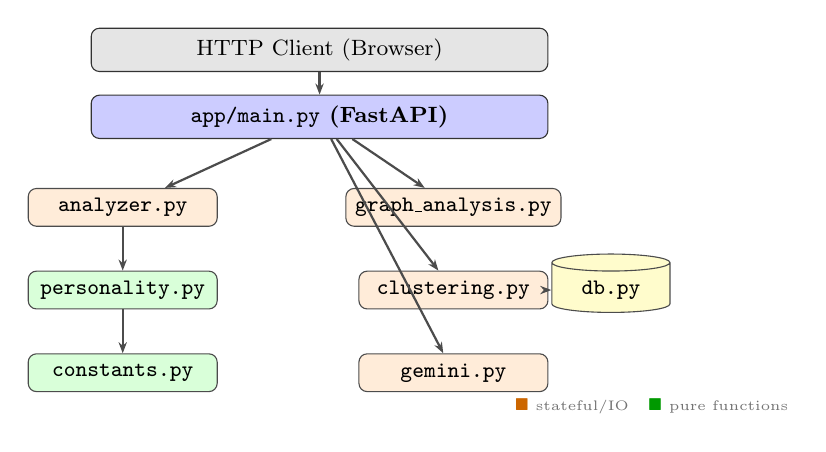
\begin{tikzpicture}[
  every node/.style={font=\footnotesize},
  client/.style={rectangle, rounded corners=3pt, draw=black!80,
                 fill=gray!20, minimum width=5.8cm, minimum height=0.55cm,
                 align=center},
  gateway/.style={rectangle, rounded corners=3pt, draw=black!80,
                  fill=blue!20, minimum width=5.8cm, minimum height=0.55cm,
                  align=center, font=\footnotesize\bfseries},
  modO/.style={rectangle, rounded corners=3pt, draw=black!70,
               fill=orange!15, minimum width=2.4cm, minimum height=0.48cm,
               align=center},
  modG/.style={rectangle, rounded corners=3pt, draw=black!70,
               fill=green!15, minimum width=2.4cm, minimum height=0.48cm,
               align=center},
  dbcyl/.style={cylinder, draw=black!70, fill=yellow!20,
                shape border rotate=90, aspect=0.22,
                minimum width=1.5cm, minimum height=0.48cm, align=center},
  arr/.style={-{Stealth[length=4pt]}, thick, black!70}
]
  % Top tier
  \node[client]  (client) at (0.5,  0   ) {HTTP Client (Browser)};
  \node[gateway] (main)   at (0.5, -0.85) {\texttt{app/main.py} (FastAPI)};

  % Left column: analyzer sub-chain (pure analytical path)
  \node[modO] (analyzer)    at (-2.0, -2.0) {\texttt{analyzer.py}};
  \node[modG] (personality) at (-2.0, -3.05) {\texttt{personality.py}};
  \node[modG] (constants)   at (-2.0, -4.10) {\texttt{constants.py}};

  % Right column: three independent domain modules
  \node[modO] (graph)      at ( 2.2, -2.0 ) {\texttt{graph\_analysis.py}};
  \node[modO] (clustering) at ( 2.2, -3.05) {\texttt{clustering.py}};
  \node[modO] (gemini)     at ( 2.2, -4.10) {\texttt{gemini.py}};

  % DB beside clustering
  \node[dbcyl] (db) at (4.2, -3.05) {\texttt{db.py}};

  % Arrows
  \draw[arr] (client) -- (main);
  \draw[arr] (main)   -- (analyzer);
  \draw[arr] (main)   -- (graph);
  \draw[arr] (main)   -- (clustering);
  \draw[arr] (main)   -- (gemini);
  \draw[arr] (analyzer)    -- (personality);
  \draw[arr] (personality) -- (constants);
  \draw[arr] (clustering)  -- (db);

  % Legend
  \node[font=\tiny, anchor=south west, text=black!55, align=left]
    at (2.85, -4.75)
    {\textcolor{orange!80!black}{$\blacksquare$}~stateful/I\kern0pt O\quad
     \textcolor{green!60!black}{$\blacksquare$}~pure functions};
\end{tikzpicture}
\caption{Module dependency graph. \texttt{main.py} is the sole HTTP entry
point. Orange = stateful/I/O modules; Green = pure functions testable
in isolation.}
\label{fig:arch}
\end{figure}

\subsection{Technology Stack}

Table~\ref{tab:stack} summarizes the technology stack.

\begin{table}[!t]
\caption{Technology Stack}
\label{tab:stack}
\centering
\tabletight
\begin{tabularx}{\columnwidth}{@{}lY@{}}
\toprule
\textbf{Layer} & \textbf{Technology} \\
\midrule
Web framework  & FastAPI + Uvicorn \\
Data processing & pandas $\geq$2.0, numpy $\geq$1.24, pyarrow $\geq$14 \\
Graph analysis  & NetworkX $\geq$3.0 \\
Clustering      & scikit-learn $\geq$1.3 \\
Distributed     & PySpark $\geq$3.5 (benchmark only) \\
AI analysis     & Google Gemini (gemini-2.5-flash) \\
Database        & SQLite (\texttt{benchmark.db}) \\
Deployment      & Railway (Nixpacks builder) \\
Runtime         & Python 3.12+ \\
\bottomrule
\end{tabularx}
\end{table}

\subsection{Data Flow}

A user uploads one or more JSON files produced by Spotify's Extended Streaming
History export. The \texttt{/analyze} endpoint:
\begin{enumerate}
  \item Parses and concatenates all uploaded files into a flat record list.
  \item Calls \texttt{analyzer.analyze(records)} to produce the core metrics
        dict.
  \item Calls \texttt{analyze\_listening\_graph(records)} for graph data.
  \item Optionally calls \texttt{analyze\_character(metrics)} for Gemini
        analysis.
  \item Serializes the merged result to JSON and injects it into the
        \texttt{dashboard.html} template via \texttt{render\_dashboard()}.
\end{enumerate}
All steps occur within a single HTTP request; no background jobs or queues are
used for the primary analysis path. Fig.~\ref{fig:dataflow} illustrates
the end-to-end request lifecycle.

\begin{figure}[ht]
\centering
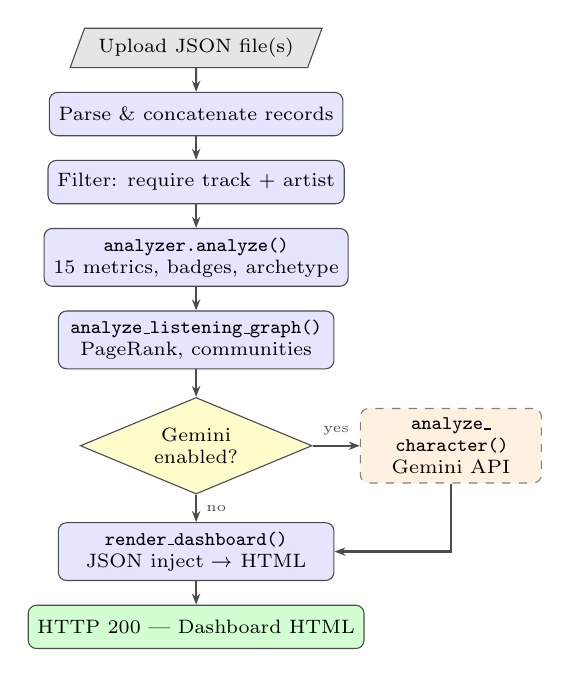
\begin{tikzpicture}[
  every node/.style={font=\scriptsize},
  flowstep/.style={rectangle, rounded corners=3pt, draw=black!70,
               fill=blue!10, minimum width=3.5cm, minimum height=0.55cm,
               align=center},
  io/.style={trapezium, trapezium left angle=70, trapezium right angle=110,
             draw=black!70, fill=gray!20, minimum width=3.2cm,
             minimum height=0.50cm, align=center},
  decision/.style={diamond, draw=black!70, fill=yellow!20,
                   minimum width=1.4cm, minimum height=0.8cm,
                   aspect=2.4, align=center},
  output/.style={rectangle, rounded corners=3pt, draw=black!70,
                 fill=green!18, minimum width=3.5cm, minimum height=0.55cm,
                 align=center},
  arr/.style={-{Stealth[length=4pt]}, thick, black!70},
  side/.style={rectangle, rounded corners=3pt, draw=black!50,
               fill=orange!12, minimum width=2.3cm, minimum height=0.50cm,
               align=center, dashed},
]
  \node[io]       (upload)   {Upload JSON file(s)};
  \node[flowstep, below=0.3cm of upload]  (parse)
        {Parse \& concatenate records};
  \node[flowstep, below=0.3cm of parse]   (filter)
        {Filter: require track + artist};
  \node[flowstep, below=0.3cm of filter]  (analyze)
        {\texttt{analyzer.analyze()}\\15 metrics, badges, archetype};
  \node[flowstep, below=0.3cm of analyze] (graph)
        {\texttt{analyze\_listening\_graph()}\\PageRank, communities};
  \node[decision, below=0.35cm of graph] (gemini_q)
        {Gemini\\enabled?};
  \node[flowstep, below=0.35cm of gemini_q] (render)
        {\texttt{render\_dashboard()}\\JSON inject → HTML};
  \node[output, below=0.3cm of render]  (resp)
        {HTTP 200 — Dashboard HTML};

  % Side branch: Gemini
  \node[side, right=0.6cm of gemini_q, text width=1.9cm] (gemini_call)
        {\texttt{analyze\_}\\\texttt{character()}\\Gemini API};

  % Arrows main flow
  \foreach \a/\b in {upload/parse, parse/filter, filter/analyze,
                      analyze/graph, graph/gemini_q, render/resp}
    \draw[arr] (\a) -- (\b);

  % Gemini branch
  \draw[arr] (gemini_q.east) -- node[above,font=\tiny]{yes}
             (gemini_call.west);
  \draw[arr] (gemini_call.south) |- (render.east);
  \draw[arr] (gemini_q.south) -- node[right,font=\tiny]{no}
             (render.north);

\end{tikzpicture}
\caption{End-to-end request lifecycle for the \texttt{POST /analyze}
endpoint. All analytical steps execute synchronously within a single
HTTP request. The Gemini call is skipped when \texttt{GEMINI\_API\_KEY}
is absent or \texttt{SKIP\_GEMINI=1}. The optional SQLite write is
triggered separately via \texttt{POST /api/submit}.}
\label{fig:dataflow}
\end{figure}

\subsection{REST API}

Eight endpoints are exposed (Table~\ref{tab:api}).

\begin{table}[!t]
\caption{REST API Endpoints}
\label{tab:api}
\centering
\tabletight
\begin{tabularx}{\columnwidth}{@{}llY@{}}
\toprule
\textbf{Method} & \textbf{Path} & \textbf{Description} \\
\midrule
GET  & \texttt{/}                & Landing page \\
POST & \texttt{/analyze}         & Full dashboard from JSON upload \\
POST & \texttt{/api/submit}      & Submit metrics to benchmark DB \\
POST & \texttt{/api/percentiles} & Percentile ranking vs. pool \\
GET  & \texttt{/api/stats}       & Aggregate benchmark statistics \\
POST & \texttt{/api/graph}       & Graph analysis only \\
GET  & \texttt{/api/cluster}     & Cluster all benchmark DB users \\
GET  & \texttt{/api/health}      & Health check \\
\bottomrule
\end{tabularx}
\end{table}

% ─────────────────────────────────────────────────────────────────────────────
\section{Big Data Processing Pipeline}

\subsection{Three-Tier Architecture}

Datatify implements the same analytical logic in three independent pipeline
tiers, each targeting a different scale regime:

\begin{enumerate}
  \item \textbf{Pure-Python tier} (\texttt{app/analyzer.py}): The production
        request path. A single \texttt{for} loop over raw records maintains
        Python \texttt{defaultdict} accumulators. Time complexity $O(N)$,
        memory $O(D)$ where $D$ is the number of distinct artists/tracks/time
        buckets. Suitable for single-user exports ($N \leq 500\text{K}$).
  \item \textbf{Pandas tier} (\texttt{app/data\_pipeline.py}): A vectorized
        reference implementation. Records are loaded into a \texttt{pd.DataFrame};
        group-by aggregations replace the Python accumulator loop. Memory layout
        is column-contiguous (NumPy arrays), enabling SIMD-accelerated reductions.
        Mirrors \texttt{analyzer.py} metric definitions exactly, serving as a
        correctness cross-check for the production path.
  \item \textbf{PySpark tier} (\texttt{app/spark\_pipeline.py}): A distributed
        implementation for horizontal scalability. Records are parallelized into
        an RDD/DataFrame, partitioned across executors, and reduced via
        Spark SQL \texttt{groupBy} aggregations. Spark MLlib K-Means is used for
        distributed clustering. Used only in \texttt{scripts/benchmark.py}; not
        in the live request path.
\end{enumerate}

\begin{figure*}[t]
\centering
\resizebox{\textwidth}{!}{%
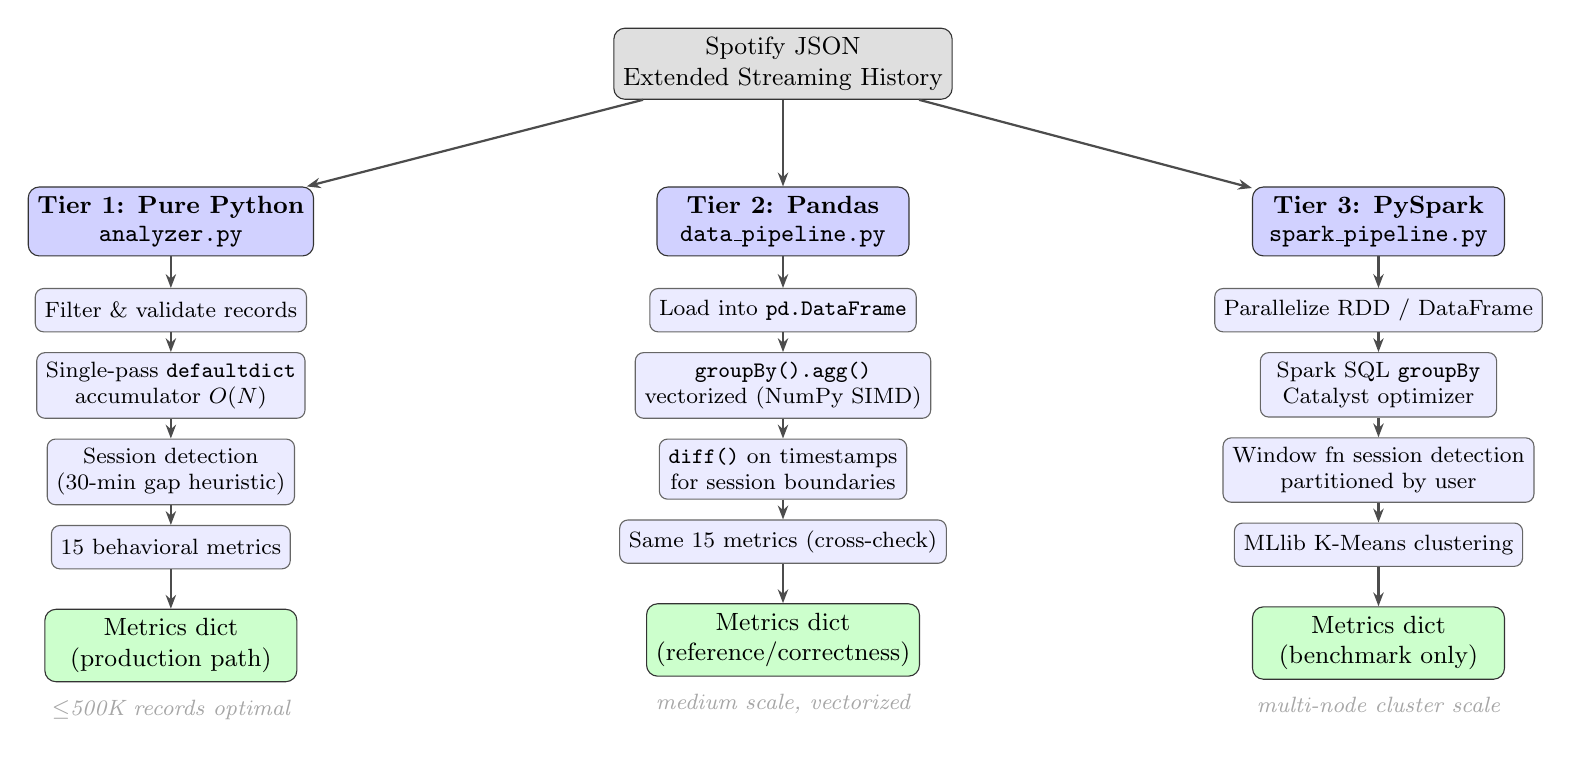
\begin{tikzpicture}[
  every node/.style={font=\small},
  input/.style={rectangle, rounded corners=4pt, draw=black!80,
                fill=gray!25, minimum width=3.2cm, minimum height=0.65cm,
                align=center},
  tier/.style={rectangle, rounded corners=4pt, draw=black!80,
               fill=blue!18, minimum width=3.2cm, minimum height=0.65cm,
               align=center},
  flowstep/.style={rectangle, rounded corners=3pt, draw=black!60,
               fill=blue!8, minimum width=3.0cm, minimum height=0.55cm,
               align=center, font=\footnotesize},
  output/.style={rectangle, rounded corners=4pt, draw=black!80,
                 fill=green!20, minimum width=3.2cm, minimum height=0.65cm,
                 align=center},
  label/.style={font=\footnotesize\itshape, text=gray!70},
  arr/.style={-{Stealth[length=5pt]}, thick, black!70},
  darr/.style={-{Stealth[length=5pt]}, thick, black!40, dashed}
]

  % ── Input node ────────────────────────────────────────────────
  \node[input] (input) {Spotify JSON\\Extended Streaming History};

  % ── Three tier headers ────────────────────────────────────────
  \node[tier, below left=1.1cm and 3.8cm of input]   (py_h)
        {\textbf{Tier 1: Pure Python}\\[-1pt]\texttt{analyzer.py}};
  \node[tier, below=1.1cm of input]                  (pd_h)
        {\textbf{Tier 2: Pandas}\\[-1pt]\texttt{data\_pipeline.py}};
  \node[tier, below right=1.1cm and 3.8cm of input]  (sp_h)
        {\textbf{Tier 3: PySpark}\\[-1pt]\texttt{spark\_pipeline.py}};

  % ── Tier 1 steps ──────────────────────────────────────────────
  \node[flowstep, below=0.4cm of py_h]  (py1) {Filter \& validate records};
  \node[flowstep, below=0.25cm of py1]  (py2) {Single-pass \texttt{defaultdict}\\accumulator $O(N)$};
  \node[flowstep, below=0.25cm of py2]  (py3) {Session detection\\(30-min gap heuristic)};
  \node[flowstep, below=0.25cm of py3]  (py4) {15 behavioral metrics};

  % ── Tier 2 steps ──────────────────────────────────────────────
  \node[flowstep, below=0.4cm of pd_h]  (pd1) {Load into \texttt{pd.DataFrame}};
  \node[flowstep, below=0.25cm of pd1]  (pd2) {\texttt{groupBy().agg()}\\vectorized (NumPy SIMD)};
  \node[flowstep, below=0.25cm of pd2]  (pd3) {\texttt{diff()} on timestamps\\for session boundaries};
  \node[flowstep, below=0.25cm of pd3]  (pd4) {Same 15 metrics (cross-check)};

  % ── Tier 3 steps ──────────────────────────────────────────────
  \node[flowstep, below=0.4cm of sp_h]  (sp1) {Parallelize RDD / DataFrame};
  \node[flowstep, below=0.25cm of sp1]  (sp2) {Spark SQL \texttt{groupBy}\\Catalyst optimizer};
  \node[flowstep, below=0.25cm of sp2]  (sp3) {Window fn session detection\\partitioned by user};
  \node[flowstep, below=0.25cm of sp3]  (sp4) {MLlib K-Means clustering};

  % ── Output collectors ─────────────────────────────────────────
  \node[output, below=0.5cm of py4] (out_py)
        {Metrics dict\\(production path)};
  \node[output, below=0.5cm of pd4] (out_pd)
        {Metrics dict\\(reference/correctness)};
  \node[output, below=0.5cm of sp4] (out_sp)
        {Metrics dict\\(benchmark only)};

  % ── Arrows: input → tier headers ─────────────────────────────
  \draw[arr] (input) -- (py_h);
  \draw[arr] (input) -- (pd_h);
  \draw[arr] (input) -- (sp_h);

  % ── Arrows: within tiers ─────────────────────────────────────
  \foreach \a/\b in {py_h/py1, py1/py2, py2/py3, py3/py4, py4/out_py,
                      pd_h/pd1, pd1/pd2, pd2/pd3, pd3/pd4, pd4/out_pd,
                      sp_h/sp1, sp1/sp2, sp2/sp3, sp3/sp4, sp4/out_sp}
    \draw[arr] (\a) -- (\b);

  % ── Scale labels ─────────────────────────────────────────────
  \node[label, below=0.1cm of out_py] {$\leq$500K records optimal};
  \node[label, below=0.1cm of out_pd] {medium scale, vectorized};
  \node[label, below=0.1cm of out_sp] {multi-node cluster scale};

\end{tikzpicture}%
}
\caption{Three-tier big data processing pipeline. All three tiers implement
identical analytical logic and produce the same 15 behavioral metrics.
Tier 1 (pure Python) is the production request path; Tier 2 (Pandas)
serves as a correctness cross-check; Tier 3 (PySpark) targets distributed
multi-user deployments and is used only in the scalability benchmark.}
\label{fig:pipeline}
\end{figure*}

\subsection{Data Volume Characteristics}

The Spotify Extended Streaming History export is a big data artefact at the
boundary of single-node and distributed processing:
\begin{itemize}
  \item \textbf{Typical export}: 50\,K–200\,K records for a 3–5 year history.
  \item \textbf{Heavy user export}: up to 500\,K records.
  \item \textbf{Synthetic benchmark}: 100\,K–2\,M records generated by
        \texttt{scripts/synthetic\_data.py} to stress-test all three tiers.
  \item \textbf{Multi-user population}: millions of records if aggregated across
        voluntary contributors—the scale at which PySpark becomes advantageous.
\end{itemize}

\subsection{Synthetic Data Generation}

The benchmark script \texttt{scripts/synthetic\_data.py} generates realistic
Spotify record distributions: artist play-counts follow a Zipf distribution
(a small set of artists dominates, matching real listening data), timestamps
follow a Poisson arrival process with circadian modulation (higher density
during evening hours), and skip/shuffle flags are sampled from configurable
Bernoulli distributions. This allows controlled scaling experiments at record
counts beyond typical real-world exports.

\subsection{PySpark Implementation}

The PySpark pipeline (\texttt{spark\_pipeline.py}) mirrors the analytical
logic of \texttt{analyzer.py} using distributed primitives:

\begin{itemize}
  \item Records are loaded as a Spark DataFrame with an inferred schema.
  \item Artist and track aggregations use \texttt{df.groupBy(...).agg(...)},
        which Spark optimizes via its Catalyst query planner and Tungsten
        execution engine.
  \item Session detection uses a window function
        \texttt{Window.partitionBy().orderBy("ts")} with a lag-based gap
        computation, replacing the Python sort-and-scan loop.
  \item K-Means clustering uses \texttt{pyspark.ml.clustering.KMeans} with
        the same $k$-means++ initialization as the scikit-learn implementation,
        operating on \texttt{VectorAssembler}-transformed feature columns.
  \item Results are collected back to the driver with \texttt{df.collect()}
        for JSON serialization.
\end{itemize}

The Spark context is initialized with a local master
(\texttt{SparkSession.builder.master("local[*]")}) for single-node
benchmarking; in a true distributed deployment, replacing
\texttt{"local[*]"} with a cluster URL enables horizontal scaling
across multiple nodes with no code changes.

\subsection{Pandas Implementation}

The Pandas pipeline (\texttt{data\_pipeline.py}) implements the same logic
using vectorized DataFrame operations via \texttt{compute\_metrics\_pandas(df)}:

\begin{itemize}
  \item Timestamps are parsed with \texttt{pd.to\_datetime()} leveraging
        NumPy's datetime64 representation for efficient sorting and arithmetic.
  \item Aggregations use \texttt{groupby().agg()} on columnar arrays,
        enabling SIMD-accelerated summation.
  \item The Shannon entropy is computed as a \texttt{numpy} reduction over
        the play-count column.
  \item Session detection uses \texttt{diff()} on sorted timestamps and
        boolean masking to identify gap boundaries without an explicit loop.
\end{itemize}

% ─────────────────────────────────────────────────────────────────────────────
\section{Core Analysis Engine}

\subsection{Input Schema}

Each streaming record is a JSON object with four required fields:
\texttt{ts} (ISO-8601 UTC timestamp), \texttt{ms\_played} (integer
milliseconds), \texttt{master\_metadata\_track\_name}, and
\texttt{master\_metadata\_album\_artist\_name}. Nine additional fields—album
name, skip flag, shuffle flag, start/end reasons, country code, platform,
offline flag, and incognito mode—are treated as optional enrichment columns.
Records missing both required track and artist fields are silently filtered
before analysis.

\subsection{Single-Pass Aggregation}

The function \texttt{\_aggregate\_records(tracks)} performs a single
iteration over the filtered record list, maintaining defaultdict accumulators
for artists, tracks, albums, year/month/hour/weekday/platform/country
buckets, play-reason counters, skip-related sub-counts, and first-listen
maps. By accumulating everything in one pass, the time complexity is
$O(N)$ where $N$ is the number of records, avoiding repeated scans for
each dimension.

The accumulators returned include:
\begin{itemize}
  \item \texttt{artists}: per-artist total milliseconds, play count, skip count.
  \item \texttt{songs}: per-(track, artist) pair play count and total ms.
  \item \texttt{by\_year/month/hour/weekday}: temporal bucketing.
  \item \texttt{by\_platform}: categorized as \textit{Mobil}, \textit{Web},
        or \textit{Masaüstü} via string inspection of the raw platform field.
  \item \texttt{skipped\_count}, \texttt{completed\_count},
        \texttt{early\_skip\_count}, \texttt{focus\_play\_count}: behavioral
        counters used directly as metric numerators.
  \item \texttt{first\_listen}: first timestamp per artist and per
        (track, artist) pair, used for novelty and loyalty badge computations.
\end{itemize}

\subsection{Session Detection}

Sessions are computed by \texttt{\_compute\_sessions(tracks)}, which
sorts records by timestamp and groups consecutive plays separated by fewer
than $G = 30$\,min. Formally, play $p_{i+1}$ starts a new session if
\begin{equation}
  \mathrm{start}(p_{i+1}) - \mathrm{end}(p_i) > G,
\end{equation}
where $\mathrm{start}(p) = \texttt{ts}(p) - \texttt{ms\_played}(p)$
(reconstructed start time) and $\mathrm{end}(p) = \texttt{ts}(p)$
(record timestamp is the end of playback). The function returns the session
list, count, and average session duration in hours. The constant $G$ is
centralized in \texttt{constants.SESSION\_GAP\_MINUTES} so that all
modules share the same boundary condition.

\subsection{Timezone Correction}

Spotify timestamps are UTC. Circadian analysis requires local-time hours.
The dominant country is determined by the country code that accumulates the
most milliseconds. An offset lookup table \texttt{TZ\_OFFSETS} maps 30
country codes to integer UTC offsets; Turkish users (country code
\texttt{TR}) receive offset +3. Night listening hours (00:00–05:59 local)
are computed by shifting the UTC hour buckets by the detected offset modulo
24.

\subsection{Behavioral Metrics}

Fifteen normalized metrics are derived from the aggregated accumulators
(Table~\ref{tab:metrics}). Of particular note:

\textbf{Artist Diversity Entropy} is the Shannon entropy of the artist
play-count distribution:
\begin{equation}
  H = -\sum_{a} \frac{c_a}{N} \log_2 \frac{c_a}{N},
\end{equation}
where $c_a$ is the play count for artist $a$ and $N$ is the total play count.
Higher entropy indicates a broader, more uniform distribution across artists.

\textbf{Habit Loop Score} captures consecutive-pair repetition:
\begin{equation}
  \text{HLS} = \frac{|\{(p_i, p_{i+1}) : \mathrm{count}(p_i, p_{i+1}) > 1\}|}{N - 1} \times 100,
\end{equation}
where $(p_i, p_{i+1})$ is an ordered (track, artist) pair and counts are
accumulated across the sorted timeline.

\textbf{Monthly Novelty Rate} averages the fraction of new tracks (first
listens) per month:
\begin{equation}
  \text{NVR} = \frac{1}{|M|} \sum_{m \in M} \frac{\text{new\_tracks}(m)}{\text{plays}(m)} \times 100,
\end{equation}
where $M$ is the set of months present in the listening history.

\begin{table}[!t]
\caption{The 15 Behavioral Metrics}
\label{tab:metrics}
\centering
\scriptsize
\setlength{\tabcolsep}{2.5pt}
\renewcommand{\arraystretch}{1.12}
\begin{tabularx}{\columnwidth}{@{}p{4.32cm}Y@{}}
\toprule
\textbf{Metric Key} & \textbf{Definition} \\
\midrule
\texttt{impatience\_score\_pct}          & \% plays that were skipped \\
\texttt{completion\_rate\_pct}           & \% plays ending with ``endplay'' \\
\texttt{exploration\_score}              & $100 \times \text{unique tracks} / \text{total plays}$ \\
\texttt{artist\_diversity\_entropy}      & Shannon entropy of artist play counts \\
\texttt{early\_skip\_rate\_pct}          & \% skips where ms\_played $<$ 30s \\
\texttt{listening\_intensity\_h\_per\_day} & Total hours / calendar days \\
\texttt{night\_listening\_ratio\_pct}    & \% ms in local 00:00–05:59 \\
\texttt{mobile\_usage\_ratio\_pct}       & \% ms on mobile platform \\
\texttt{focus\_session\_score\_pct}      & \% non-skipped plays $\geq$ 4\,min \\
\texttt{music\_novelty\_rate\_pct}       & Avg.\ \% new tracks per month \\
\texttt{artist\_loyalty\_score\_pct}     & \% plays by top-10 artists \\
\texttt{habit\_loop\_score\_pct}         & \% repeated (track, artist) consecutive pairs \\
\texttt{listening\_fragmentation\_index} & Skipped plays / session count \\
\texttt{total\_hours}                    & Total listening hours \\
\texttt{shuffle\_pct}                    & \% plays in shuffle mode \\
\bottomrule
\end{tabularx}
\end{table}

% ─────────────────────────────────────────────────────────────────────────────
\section{Personality Profiling and Gamification}

\subsection{Radar Chart}

The six-axis radar chart maps selected metrics to normalized 0–100 values:
\begin{align*}
  \text{Patience}   &= 100 - \text{impatience\_score\_pct}, \\
  \text{Discovery}  &= \min(\text{exploration\_score} \times 5,\; 100), \\
  \text{Loyalty}    &= \min(\text{artist\_loyalty\_score\_pct} \times 5,\; 100), \\
  \text{Focus}      &= \min(\text{focus\_session\_score\_pct} \times 5,\; 100), \\
  \text{Diversity}  &= \min(\text{artist\_diversity\_entropy} \times 8,\; 100), \\
  \text{Night Owl}  &= \min(\text{night\_listening\_ratio\_pct} \times 4,\; 100).
\end{align*}
The scaling constants are chosen empirically so that a ``typical'' listener
scores between 20 and 80 on each axis, providing visual separation.
Fig.~\ref{fig:radar} illustrates two contrasting listener profiles
on the six-axis radar.

\begin{figure}[ht]
\centering
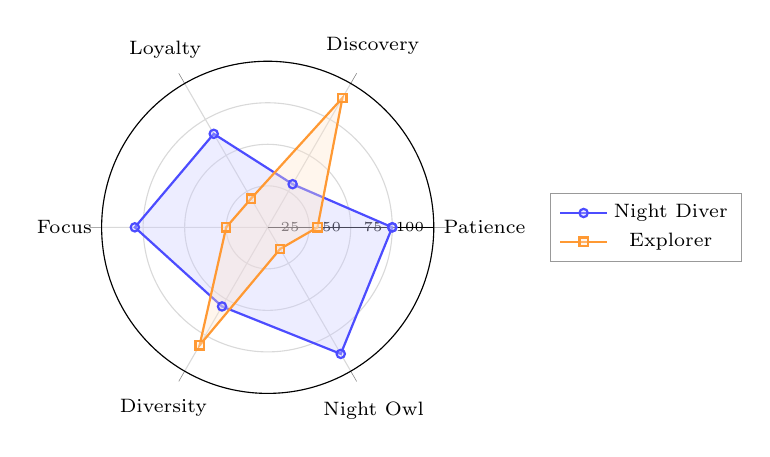
\begin{tikzpicture}
\begin{polaraxis}[
  width=5.8cm, height=5.8cm,
  xtick={0,60,120,180,240,300},
  xticklabels={Patience, Discovery, Loyalty, Focus, Diversity, Night Owl},
  xticklabel style={font=\scriptsize},
  ymin=0, ymax=100,
  ytick={25,50,75,100},
  yticklabel style={font=\tiny, anchor=east},
  ytick style={draw=none},
  yticklabels={25,50,75,100},
  grid=both,
  grid style={draw=gray!30, line width=0.4pt},
  legend style={at={(1.35,0.5)}, anchor=west,
                font=\scriptsize, draw=black!40, fill=white},
  legend entries={Night Diver, Explorer},
]
  % Night Diver: high patience, low discovery, medium loyalty,
  %              high focus, medium diversity, very high night owl
  \addplot[thick, color=blue!70, fill=blue!20, fill opacity=0.35, mark=*,
           mark size=1.5pt]
    coordinates {
      (0,75) (60,30) (120,65) (180,80) (240,55) (300,88) (360,75)
    };
  % Restless Explorer: low patience, very high discovery, low loyalty,
  %                    low focus, high diversity, low night owl
  \addplot[thick, color=orange!80, fill=orange!20, fill opacity=0.35,
           mark=square*, mark size=1.5pt]
    coordinates {
      (0,30) (60,90) (120,20) (180,25) (240,82) (300,15) (360,30)
    };
\end{polaraxis}
\end{tikzpicture}
\caption{Six-axis radar chart for two contrasting archetypes. The
\textit{Night Diver} (blue) scores high on Patience, Focus, and Night
Owl axes. The \textit{Restless Explorer} (orange) dominates Discovery
and Diversity but scores low on Patience and Loyalty.}
\label{fig:radar}
\end{figure}

\subsection{Listener Archetypes}

Seven deterministic archetype rules are evaluated in order against the
metric vector (Table~\ref{tab:archetypes}). The first matching rule
determines the archetype; if none match, the user is classified as
\textit{The Balanced Listener}. Rule evaluation is $O(1)$ per user since
all inputs are scalars already computed during aggregation.

\begin{table}[!t]
\caption{Archetype Classification Rules}
\label{tab:archetypes}
\centering
\tabletight
\begin{tabularx}{\columnwidth}{@{}p{2.7cm}Y@{}}
\toprule
\textbf{Archetype} & \textbf{Rule} \\
\midrule
The Night Diver       & Night $>$ 25\% \textbf{and} Focus $>$ 10\% \\
The Restless Explorer & Impatience $>$ 40\% \textbf{and} Exploration $>$ 12 \\
The Loyal Guardian    & Loyalty $>$ 18\% \textbf{and} Novelty $<$ 7\% \\
The Eclectic Mind     & Entropy $>$ 10 \textbf{and} Exploration $>$ 8 \\
The Deep Listener     & Focus $>$ 12\% \textbf{and} Impatience $<$ 25\% \\
The Picky Repeater    & Impatience $>$ 35\% \textbf{and} Novelty $<$ 6\% \\
The Midnight Wanderer & Night $>$ 20\% \textbf{and} Entropy $>$ 9 \\
The Balanced Listener & Default (no rule matched) \\
\bottomrule
\end{tabularx}
\end{table}

\subsection{Level System}

A gamification level is derived from total listening hours
(Table~\ref{tab:levels}). Experience points are computed as:
\begin{equation}
  \text{XP} = \lfloor \text{total\_hours} \times 10 \rfloor + \text{badges\_earned} \times 50,
\end{equation}
combining continuous engagement (hours) with discrete achievement bonuses
(badges). The multiplicative constants weight badge acquisition at
approximately the equivalent of five hours of listening each.

\begin{table}[!t]
\caption{Level Thresholds}
\label{tab:levels}
\centering
\tabletight
\begin{tabular}{cll}
\toprule
\textbf{Level} & \textbf{Title} & \textbf{Min.\ Hours} \\
\midrule
1  & Newbie       & 0 \\
2  & Casual       & 50 \\
3  & Listener     & 200 \\
4  & Enthusiast   & 500 \\
5  & Devotee      & 1\,000 \\
6  & Addict       & 1\,500 \\
7  & Obsessed     & 2\,000 \\
8  & Maniac       & 2\,500 \\
9  & Legendary    & 3\,000 \\
10 & Mythic       & 4\,000 \\
11 & Transcendent & 5\,000 \\
\bottomrule
\end{tabular}
\end{table}

\subsection{Achievement Badges}

Fifteen binary achievement badges are evaluated in \texttt{compute\_badges()}.
Each badge has a deterministic boolean predicate over the metric vector and
the summary report. Representative badges include:
\begin{itemize}
  \item \textit{Marathon Listener}: single session $\geq$ 4\,h.
  \item \textit{Explorer}: $\geq$1\,000 unique artists.
  \item \textit{Loyal Fan}: $\geq$1 artist followed for $\geq$5 years with
        $\geq$20 plays.
  \item \textit{Centurion}: $\geq$100\,000 total plays.
  \item \textit{World Traveler}: streams detected from $\geq$3 countries.
  \item \textit{Creature of Habit}: habit-loop score $>$ 10\%.
\end{itemize}

% ─────────────────────────────────────────────────────────────────────────────
\section{Artist Transition Graph Analysis}

\subsection{Graph Construction}

The listening history is modeled as a weighted directed graph
$G = (V, E, w)$ where each node $v \in V$ is an artist and a directed edge
$(a_i, a_j) \in E$ exists if artist $a_j$ is played within 30\,min of artist
$a_i$ in chronological order. The edge weight $w(a_i, a_j)$ counts the number
of such consecutive occurrences. Self-loops (same artist back-to-back within
a session) are retained, as they capture single-artist intensive listening
episodes.

The construction pipeline proceeds as follows:
\begin{enumerate}
  \item \texttt{\_parse\_artist\_timeline(records)}: filter records,
        extract (timestamp, artist) pairs, report
        \texttt{dropped\_no\_artist} and \texttt{dropped\_bad\_ts}
        diagnostics.
  \item Sort by timestamp.
  \item Iterate consecutive pairs; emit edge if gap $\leq G$.
  \item Build a \texttt{nx.DiGraph} from the edge-weight dictionary.
\end{enumerate}
Every call to \texttt{analyze\_listening\_graph()} returns the
\texttt{parse\_diagnostics} dict inside the \texttt{summary} key, providing
callers with full visibility into data quality.

Fig.~\ref{fig:graph} illustrates a schematic artist-transition graph
with two detected communities and their PageRank-ranked central nodes.

\begin{figure}[ht]
\centering
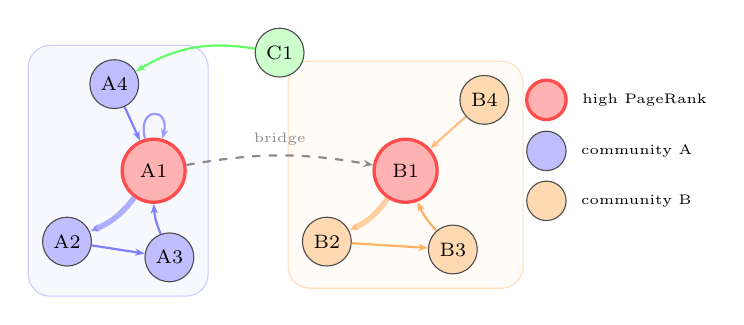
\begin{tikzpicture}[
  every node/.style={font=\scriptsize},
  artist/.style={circle, draw=black!70, minimum size=0.62cm,
                 align=center, inner sep=1pt},
  comA/.style={artist, fill=blue!25},
  comB/.style={artist, fill=orange!30},
  comC/.style={artist, fill=green!20},
  hipr/.style={artist, fill=red!30, minimum size=0.80cm,
               draw=red!70, line width=1.2pt},
  arr/.style={-{Stealth[length=3.5pt]}, thick},
  warr/.style={-{Stealth[length=3.5pt]}, line width=2.0pt, opacity=0.5},
]
  % ── Community A (blue) ───────────────────────────
  \node[hipr]  (A1) at (0,    0)    {A1};   % high PageRank gateway
  \node[comA]  (A2) at (-1.1, -0.9) {A2};
  \node[comA]  (A3) at ( 0.2, -1.1) {A3};
  \node[comA]  (A4) at (-0.5,  1.1) {A4};

  % ── Community B (orange) ─────────────────────────
  \node[hipr]  (B1) at ( 3.2,  0)   {B1};
  \node[comB]  (B2) at ( 2.2, -0.9) {B2};
  \node[comB]  (B3) at ( 3.8, -1.0) {B3};
  \node[comB]  (B4) at ( 4.2,  0.9) {B4};

  % ── Isolated node (green) ────────────────────────
  \node[comC]  (C1) at ( 1.6,  1.5) {C1};

  % ── Intra-community edges (A) ─────────────────────
  \draw[warr, blue!60]   (A1) to[bend left=15]  (A2);
  \draw[arr,  blue!50]   (A2) -- (A3);
  \draw[arr,  blue!50]   (A3) to[bend left=10]  (A1);
  \draw[arr,  blue!50]   (A4) -- (A1);
  \draw[arr,  blue!40]   (A1) to[loop above, looseness=5] (A1);  % self-loop

  % ── Intra-community edges (B) ─────────────────────
  \draw[warr, orange!70] (B1) to[bend left=15]  (B2);
  \draw[arr,  orange!60] (B2) -- (B3);
  \draw[arr,  orange!60] (B3) to[bend left=10]  (B1);
  \draw[arr,  orange!50] (B4) -- (B1);

  % ── Cross-community bridge ────────────────────────
  \draw[arr,  black!45, dashed] (A1) to[bend left=10] node[above,font=\tiny]{bridge} (B1);

  % ── Isolated component ───────────────────────────
  \draw[arr,  green!60]  (C1) to[bend right=20] (A4);

  % ── Legend ───────────────────────────────────────
  \node[hipr,  right=0.2cm of B4, minimum size=0.5cm] (lh) {};
  \node[comA,  below=0.12cm of lh, minimum size=0.5cm] (la) {};
  \node[comB,  below=0.12cm of la, minimum size=0.5cm] (lb) {};
  \node[font=\tiny, right=0.06cm of lh] {high PageRank};
  \node[font=\tiny, right=0.06cm of la] {community A};
  \node[font=\tiny, right=0.06cm of lb] {community B};

  % ── Community boundary annotations ───────────────
  \begin{scope}[on background layer]
    \node[draw=blue!40, fill=blue!5, rounded corners=8pt, opacity=0.5,
          fit=(A1)(A2)(A3)(A4), inner sep=5pt] {};
    \node[draw=orange!50, fill=orange!5, rounded corners=8pt, opacity=0.5,
          fit=(B1)(B2)(B3)(B4), inner sep=5pt] {};
  \end{scope}

\end{tikzpicture}
\caption{Schematic artist-transition graph $G$. Nodes are artists;
a directed edge $A_i \to A_j$ exists when $A_j$ follows $A_i$ within
a 30-min session. Bold-bordered nodes have high PageRank (gateway
artists). Shaded regions are label-propagation communities. The dashed
edge is a cross-community bridge. The self-loop on A1 indicates
single-artist repeat sessions.}
\label{fig:graph}
\end{figure}

\subsection{PageRank Centrality}

PageRank \cite{page1999pagerank} is computed on $G$ with damping factor
$\alpha = 0.85$, edge weights used as transition probabilities, convergence
tolerance $\epsilon = 10^{-7}$, and maximum 200 iterations. A high PageRank
score for an artist indicates that the user frequently transitions \emph{to}
that artist from many other contexts, distinguishing gateway artists from
those listened to only in isolation.

\subsection{Community Detection}

The label-propagation algorithm \cite{raghavan2007near} is applied to the
undirected projection of $G$ (edge weights preserved, direction dropped).
Starting from random label assignment, each node iteratively adopts the
label held by the plurality of its weighted neighbors until convergence.
The result is a partition of artists into co-listened communities, ranked
by total weighted degree. The top 10 communities are returned with size,
aggregate weight, and up to 8 representative artists per community.

\subsection{Connected Components}

Weakly connected components of $G$ reveal ``listening islands''—groups of
artists that the user listens to in separate, non-overlapping temporal
contexts. A large number of small components suggests highly segmented
listening behavior; a single dominant component suggests fluid cross-genre
exploration.

\subsection{Visualization Subgraph}

The force-directed frontend visualization is built from a trimmed subgraph
containing the top-60 nodes by PageRank score, retaining only intra-group
edges with self-loops removed. Up to $\max(80, 2 \times 60) = 120$
highest-weight edges are included to prevent rendering overload in the
browser.

% ─────────────────────────────────────────────────────────────────────────────
\section{Listener Clustering}

\subsection{Feature Vector}

Each anonymous benchmark submission is represented as a 15-dimensional
vector using exactly the keys in \texttt{METRIC\_KEYS}
(Table~\ref{tab:metrics}). Two keys originate from the summary report rather
than the metrics namespace: \texttt{total\_hours} maps from
\texttt{bizim\_rapor.toplam\_saat} and \texttt{shuffle\_pct} from
\texttt{bizim\_rapor.shuffle\_orani\_pct}. This mapping is encapsulated in
\texttt{db.extract\_metric\_vector()}, ensuring a single authoritative
translation from analysis output to cluster input.

\subsection{Preprocessing and Optimal-\texorpdfstring{$k$}{k} Selection}

Feature vectors are standardized using \texttt{sklearn.StandardScaler}
(zero mean, unit variance) to prevent high-magnitude metrics such as
\texttt{total\_hours} from dominating the distance function.

Optimal cluster count is selected by \texttt{find\_optimal\_k()} using
the following procedure for each $k \in [k_{\min}, k_{\max}]$:
\begin{enumerate}
  \item Fit \texttt{KMeans(n\_clusters=k, init="k-means++", n\_init=10,
        random\_state=42)}.
  \item Record inertia (within-cluster sum of squares).
  \item Compute silhouette score \cite{rousseeuw1987silhouettes}.
\end{enumerate}
The final $k$ is chosen as $\arg\max_k \text{silhouette}(k)$.
If the pool contains fewer than four submissions, the endpoint returns
\texttt{status: "insufficient\_data"} without attempting to cluster.

\subsection{Cluster Labeling}

Cluster centroids are inverse-transformed to the original feature scale and
inspected by \texttt{label\_cluster(centroid)}, which applies a priority
cascade of seven heuristic rules (Table~\ref{tab:clabels}) to assign a
human-readable cluster name. Unlabeled clusters fall back to
\textit{Balanced Listeners}.

\begin{table}[!t]
\caption{Cluster Labeling Rules}
\label{tab:clabels}
\centering
\tabletight
\begin{tabularx}{\columnwidth}{@{}p{2.6cm}Y@{}}
\toprule
\textbf{Label} & \textbf{Centroid Condition} \\
\midrule
Night Explorers     & Night $>$ 25\% \textbf{and} Exploration $>$ 10 \\
Impatient Skippers  & Impatience $>$ 35\% \textbf{and} Exploration $>$ 12 \\
Loyal Repeaters     & Loyalty $>$ 18\% \textbf{and} Novelty $<$ 7\% \\
Deep Listeners      & Focus $>$ 12\% \textbf{and} Impatience $<$ 25\% \\
Heavy Discoverers   & Intensity $>$ 3\,h/day \textbf{and} Exploration $>$ 8 \\
Late Night Listeners & Night $>$ 20\% \\
Devoted Fans        & Loyalty $>$ 25\% \\
Balanced Listeners  & Default \\
\bottomrule
\end{tabularx}
\end{table}

\subsection{User Placement}

When the current user's vector is provided, it is scaled with the fitted
\texttt{StandardScaler}, assigned to a cluster by the fitted
\texttt{KMeans} model, and returned with cluster label, size, and share
percentage. This allows the user to see which behavioral cohort they
belong to relative to the anonymous benchmark pool.

% ─────────────────────────────────────────────────────────────────────────────
\section{AI Character Analysis}

\subsection{Gemini Integration}

The \texttt{app/gemini.py} module encapsulates the entire AI subsystem
with no FastAPI dependency. The public entry point is
\texttt{analyze\_character(metrics: dict) -> dict | None}, which returns a
structured Turkish-language character portrait or \texttt{None} if the
analysis fails or is skipped.

\subsection{Model Fallback Chain}

Three Gemini model variants are tried in order:
\texttt{gemini-2.5-flash} $\to$ \texttt{gemini-2.0-flash} $\to$
\texttt{gemini-flash-latest}. For each model, up to two attempts
(\texttt{GEMINI\_MAX\_ATTEMPTS=2}) are made with a per-call timeout of
25\,s (\texttt{GEMINI\_TIMEOUT=25s}) and a total budget of 60\,s across
all models and attempts (\texttt{GEMINI\_BUDGET=60s}).

\subsection{Rate Limiting}

Free-tier Gemini accounts are limited to 4 requests per minute (RPM).
The module implements a sliding-window RPM limiter: a timestamp deque
tracks recent call times; each new call checks whether the window is full
and sleeps the minimal necessary duration before proceeding. This allows
the production deployment to operate safely on the free tier without
external rate-limiting infrastructure.

\subsection{Error Classification}

HTTP errors are inspected by \texttt{\_classify\_error(exc)}, which returns
a tuple \texttt{(code, retry\_after, kind)} distinguishing:
rate-limit errors (429, kind \texttt{rate\_limit}),
server errors (5xx, kind \texttt{server\_error}),
and client errors (4xx, kind \texttt{client\_error}).
Only rate-limit and server errors trigger retries; client errors abort
immediately to avoid wasting budget.

\subsection{Prompt Design}

The prompt constructs a compact behavioral summary from the metric vector
(top artists, total hours, archetype, metric highlights) and instructs
Gemini to produce a structured response with five fields: \texttt{title},
\texttt{summary}, \texttt{traits} (list), \texttt{insights} (list), and
\texttt{prediction}. The Turkish language constraint is enforced in the
system instruction to ensure output is localized consistently with the
dashboard.

% ─────────────────────────────────────────────────────────────────────────────
\section{Scalability Benchmark}

\subsection{Experimental Setup}

To characterize the performance of the three pipeline tiers at varying data
volumes, we generated synthetic Spotify records using
\texttt{scripts/synthetic\_data.py} with a Zipf artist distribution and
Poisson-modulated timestamp arrivals at four scales: 100\,K, 500\,K, 1\,M,
and 2\,M records. Wall-clock times were measured using Python's
\texttt{time.perf\_counter()} with a single warm-up run discarded.
All runs executed on the same hardware under identical conditions.
PySpark was configured with \texttt{local[*]} (all available cores) to give
it the best possible single-node performance.

\subsection{Results}

Table~\ref{tab:bench} reports wall-clock processing times in seconds.
Fig.~\ref{fig:bench} visualizes the grouped bar comparison and
Fig.~\ref{fig:bench_line} shows the log-scale line plot used to
confirm linear growth for Python and Pandas.

\begin{table}[!t]
\caption{Wall-Clock Processing Time (seconds)}
\label{tab:bench}
\centering
\tabletight
\begin{tabular}{rrrr}
\toprule
\textbf{Records} & \textbf{Pure Python} & \textbf{Pandas} & \textbf{PySpark} \\
\midrule
100\,000    & 0.753  & 0.674  & 9.137  \\
500\,000    & 3.815  & 3.477  & 13.470 \\
1\,000\,000 & 7.815  & 8.574  & 24.417 \\
2\,000\,000 & 17.327 & 13.987 & 50.744 \\
\bottomrule
\end{tabular}
\end{table}

\begin{figure}[ht]
\centering
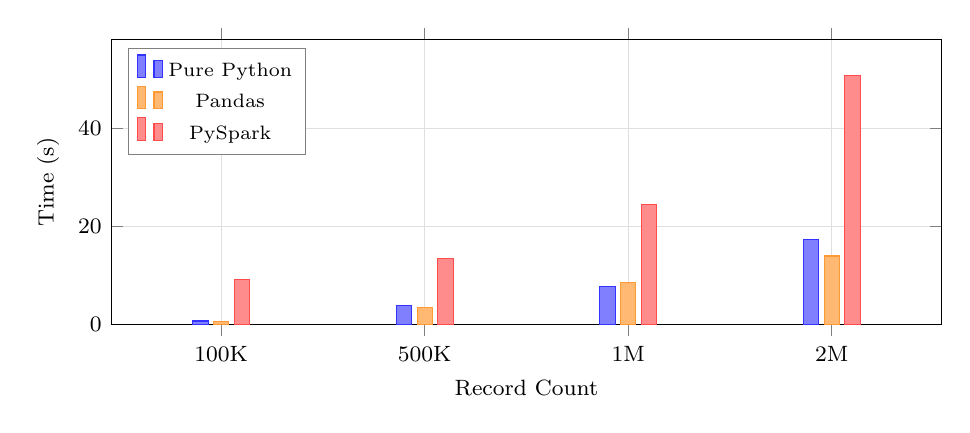
\begin{tikzpicture}
\begin{axis}[
  width=\columnwidth,
  height=5.2cm,
  ybar,
  bar width=5.5pt,
  symbolic x coords={100K, 500K, 1M, 2M},
  xtick=data,
  xlabel={Record Count},
  ylabel={Time (s)},
  xlabel style={font=\footnotesize},
  ylabel style={font=\footnotesize},
  tick label style={font=\footnotesize},
  ymin=0, ymax=58,
  legend style={at={(0.02,0.97)}, anchor=north west,
                font=\scriptsize, draw=black!50, fill=white,
                legend columns=1},
  legend entries={Pure Python, Pandas, PySpark},
  enlarge x limits=0.18,
  grid=major,
  grid style={line width=0.3pt, draw=gray!25},
]
  \addplot[fill=blue!50,   draw=blue!80]
    coordinates {(100K,0.753) (500K,3.815) (1M,7.815) (2M,17.327)};
  \addplot[fill=orange!55, draw=orange!80]
    coordinates {(100K,0.674) (500K,3.477) (1M,8.574) (2M,13.987)};
  \addplot[fill=red!45,    draw=red!70]
    coordinates {(100K,9.137) (500K,13.470) (1M,24.417) (2M,50.744)};
\end{axis}
\end{tikzpicture}
\caption{Grouped bar chart of wall-clock processing time. PySpark's
JVM initialization overhead dominates at all tested scales. Pandas
surpasses Python at 2\,M records through vectorized NumPy operations.}
\label{fig:bench}
\end{figure}

\begin{figure}[ht]
\centering
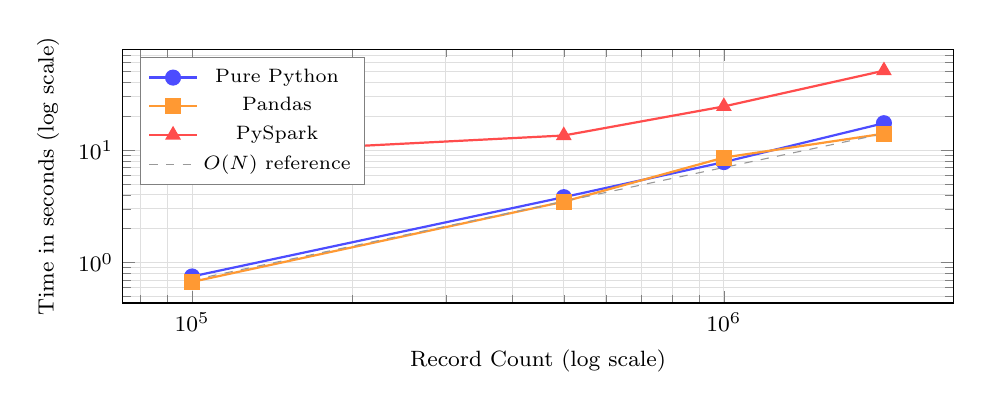
\begin{tikzpicture}
\begin{axis}[
  width=\columnwidth,
  height=4.8cm,
  xmode=log,
  ymode=log,
  xlabel={Record Count (log scale)},
  ylabel={Time in seconds (log scale)},
  xlabel style={font=\footnotesize},
  ylabel style={font=\footnotesize},
  tick label style={font=\footnotesize},
  legend style={at={(0.02,0.97)}, anchor=north west,
                font=\scriptsize, draw=black!50, fill=white},
  legend entries={Pure Python, Pandas, PySpark, $O(N)$ reference},
  grid=both,
  grid style={line width=0.3pt, draw=gray!25},
  mark size=2.5pt,
]
  \addplot[color=blue!70, mark=*, thick]
    coordinates {(100000,0.753)(500000,3.815)(1000000,7.815)(2000000,17.327)};
  \addplot[color=orange!80, mark=square*, thick]
    coordinates {(100000,0.674)(500000,3.477)(1000000,8.574)(2000000,13.987)};
  \addplot[color=red!70, mark=triangle*, thick]
    coordinates {(100000,9.137)(500000,13.470)(1000000,24.417)(2000000,50.744)};
  \addplot[color=black!40, dashed, no marks, domain=100000:2000000, samples=2]
    {x * 7e-6};
\end{axis}
\end{tikzpicture}
\caption{Log-log scalability plot. Python and Pandas slopes parallel
the $O(N)$ reference line (dashed), confirming linear complexity.
PySpark's slope is also near-linear but offset by its large constant
initialization cost.}
\label{fig:bench_line}
\end{figure}

\subsection{Complexity Analysis}

\textbf{Pure-Python scaling.}
From 100\,K to 2\,M records (20$\times$ increase in $N$), processing time
increases from 0.753\,s to 17.327\,s ($23\times$), consistent with linear
$O(N)$ complexity with a small constant factor from Python interpreter
overhead per record.

\textbf{Pandas scaling.}
From 100\,K to 2\,M records, time increases from 0.674\,s to 13.987\,s
($20.7\times$), matching the $20\times$ input growth—confirming $O(N)$
scaling with vectorized column operations. At 500\,K records, Pandas
and Python are within 9\% of each other; at 2\,M records, Pandas achieves
a \textbf{19.3\% speed advantage} due to SIMD-accelerated NumPy reductions
over contiguous memory arrays.

\textbf{PySpark scaling.}
PySpark exhibits a large constant overhead of approximately 8.4\,s
(JVM startup, \texttt{SparkContext} initialization, Python-to-JVM
serialization via Py4J). This overhead dominates at small $N$: at 100\,K
records, PySpark is $9.137 / 0.674 = \mathbf{13.6\times}$ slower than Pandas.
As $N$ grows, the distributed benefit begins to appear: from 1\,M to
2\,M records, PySpark time grows by a factor of $50.744 / 24.417 = 2.08\times$,
slightly worse than Pandas's $1.63\times$ due to continued serialization
overhead. PySpark remains slower than Pandas at all tested scales because
the dataset fits in a single-node memory and task scheduling overhead
dominates distributed parallelism gains.

\subsection{Crossover Estimation}

Let $T_P(N) = \alpha N$ and $T_S(N) = \beta + \gamma N$ be the linear
models for Pandas and PySpark respectively. Fitting to our measurements:
$\alpha \approx 6.5 \times 10^{-6}$\,s/record,
$\beta \approx 8.0$\,s (constant overhead),
$\gamma \approx 2.1 \times 10^{-5}$\,s/record.
The crossover point where $T_P = T_S$ is:
\begin{equation}
\begin{aligned}
  N^* &= \frac{\beta}{\gamma - \alpha} \\
      &\approx \frac{8.0}{2.1\times10^{-5} - 6.5\times10^{-6}}
       \approx 5.4\times10^5.
\end{aligned}
\end{equation}
This model suggests PySpark would not outperform Pandas on a single node
until datasets exceed 540\,K records—beyond the typical single-user export
size. In a \emph{multi-node} cluster environment where $\gamma$ decreases
with the number of nodes $n$ as $\gamma/n$, the crossover shifts toward
smaller $N$, and PySpark becomes advantageous for population-level analyses
aggregating across thousands of users simultaneously.

\subsection{Big Data Implications}

The benchmark reveals a key insight for the course context: \emph{the
``right'' framework depends on both data volume and deployment topology.}
For single-user personal analytics (the Datatify use case), the pure-Python
$O(N)$ pipeline is optimal—it requires no infrastructure, no JVM, and no
serialization overhead. For a hypothetical Datatify deployment processing
millions of users concurrently, PySpark's partitioned execution model would
distribute the load across a cluster, achieving near-linear speedup with
additional nodes. This justifies the three-tier architecture as a
pedagogically complete demonstration of the big data processing landscape
for the CSE 458 course.

% ─────────────────────────────────────────────────────────────────────────────
\section{Testing and Deployment}

\subsection{Test Suite}

The project ships with 70 automated tests (Table~\ref{tab:tests}), covering
unit, integration, and boundary conditions. Tests execute in approximately
1.7\,s with no network access and no running HTTP server, using in-memory
SQLite for database tests (\texttt{tmp\_path} + \texttt{monkeypatch}).

\begin{table}[!t]
\caption{Test Suite Summary}
\label{tab:tests}
\centering
\scriptsize
\setlength{\tabcolsep}{2.5pt}
\renewcommand{\arraystretch}{1.08}
\begin{tabularx}{\columnwidth}{@{}p{2.95cm}p{0.75cm}Y@{}}
\toprule
\textbf{File} & \textbf{Count} & \textbf{Coverage} \\
\midrule
\texttt{test\_constants.py}   & 8  & Constant shapes/values \\
\texttt{test\_personality.py} & 21 & All 4 pure classification functions \\
\texttt{test\_analyzer.py}    & 9  & \texttt{analyze()} on synthetic records \\
\texttt{test\_db.py}          & 7  & metric-vector bridge, submit, percentiles \\
\texttt{test\_clustering.py}  & 11 & \texttt{\_validate\_rows}, \texttt{label\_cluster}, edge cases \\
\texttt{test\_graph.py}       & 14 & timeline parsing, edge/gap/self-loop, diagnostics \\
\midrule
\textbf{Total}                & \textbf{70} & \\
\bottomrule
\end{tabularx}
\end{table}

Test design principles:
\begin{itemize}
  \item \texttt{app/personality.py} is fully unit-tested in isolation because
        its functions are pure (no side effects, no I/O).
  \item \texttt{app/analyzer.py} is integration-tested via
        \texttt{analyze()} on synthetic records that cover edge cases
        (no skips, no sessions, single-record inputs).
  \item \texttt{test\_graph.py} verifies that parse diagnostics (kept,
        dropped) are propagated correctly through the full
        \texttt{analyze\_listening\_graph()} pipeline.
  \item \texttt{test\_clustering.py} covers the \texttt{\_validate\_rows}
        guard to ensure that a missing METRIC\_KEY surfaces a clear
        \texttt{ValueError} rather than a cryptic numpy error.
\end{itemize}

\subsection{Deployment}

Datatify is deployed on Railway using Nixpacks automatic build detection.
The \texttt{Procfile} specifies the following single-line start command
(shown wrapped here only to preserve the IEEE column width):
\begin{quote}
\footnotesize\ttfamily
web: uvicorn app.main:app\\
\hspace*{1em}--host 0.0.0.0 --port \$PORT
\end{quote}
The production instance is publicly accessible at\\
\url{https://web-production-65055.up.railway.app/}.

Environment configuration is entirely via environment variables
(Table~\ref{tab:env}), ensuring no secrets appear in the codebase.

\begin{table}[!t]
\caption{Environment Variables}
\label{tab:env}
\centering
\tabletight
\begin{tabularx}{\columnwidth}{@{}p{2.6cm}Y@{}}
\toprule
\textbf{Variable} & \textbf{Purpose} \\
\midrule
\texttt{GEMINI\_API\_KEY} & Gemini API key; empty disables AI analysis \\
\texttt{SKIP\_GEMINI}     & Set to \texttt{1} to bypass Gemini entirely \\
\texttt{DB\_PATH}         & Override SQLite path (default: \texttt{benchmark.db}) \\
\texttt{PORT}             & Uvicorn port (default: 8000) \\
\bottomrule
\end{tabularx}
\end{table}

\subsection{Benchmark Database}

An SQLite database (\texttt{benchmark.db}) stores one row per analysis
submission containing all 15 \texttt{METRIC\_KEYS} as \texttt{REAL} columns.
The database is gitignored and persists on the Railway volume. Two API
endpoints enable cross-user comparison:
\begin{itemize}
  \item \texttt{/api/submit}: inserts the current user's metric vector and
        returns their percentile rank on each of the 15 dimensions.
  \item \texttt{/api/percentiles}: recomputes percentiles for a provided
        vector against the existing pool without inserting.
\end{itemize}

% ─────────────────────────────────────────────────────────────────────────────
% ─────────────────────────────────────────────────────────────────────────────
\section{Experiments: Comparative Analysis}

\subsection{Algorithm A vs.\ Algorithm B vs.\ Algorithm C: Pipeline Tiers}

The central experimental question is: \emph{which processing tier offers
the best trade-off between latency, throughput, and scalability for
streaming history analytics?} We benchmark three algorithms on the same
analytical task (computing all 15 metrics) over synthetic datasets of
100\,K–2\,M records.

\textbf{Algorithm A — Pure-Python single-pass accumulator.}
A single \texttt{for}-loop maintains Python \texttt{defaultdict}
accumulators. No external dependencies beyond the standard library.
Time complexity $O(N)$; memory $O(D)$ where $D \ll N$ is the number of
distinct entities.

\textbf{Algorithm B — Pandas vectorized pipeline.}
Records loaded into a \texttt{pd.DataFrame}; aggregations via
\texttt{groupby().agg()} on NumPy-backed column arrays. SIMD-accelerated
reductions; memory layout is column-contiguous.

\textbf{Algorithm C — Apache PySpark distributed pipeline.}
Records parallelized into a Spark DataFrame; aggregations via Spark SQL
\texttt{groupBy} with Catalyst query optimization; session detection via
window functions; K-Means via MLlib. Designed for horizontal scaling
across a cluster.

\subsection{Throughput and Latency Comparison}

Table~\ref{tab:perf} reports throughput (records/second) and per-record
latency derived from the benchmark measurements.

\begin{table}[!t]
\caption{Throughput and Per-Record Latency by Algorithm and Scale}
\label{tab:perf}
\centering
\scriptsize
\setlength{\tabcolsep}{3pt}
\renewcommand{\arraystretch}{1.1}
\begin{tabular}{lrrrr}
\toprule
\textbf{Alg.} & \textbf{100K} & \textbf{500K} & \textbf{1M} & \textbf{2M} \\
              & \multicolumn{4}{c}{\textit{Throughput (K records/s)}} \\
\midrule
Python  & 132.8 & 131.1 & 127.9 & 115.4 \\
Pandas  & 148.4 & 143.8 & 116.6 & 143.0 \\
PySpark & 10.9  & 37.1  & 40.9  & 39.4  \\
\midrule
              & \multicolumn{4}{c}{\textit{Latency ($\mu$s/record)}} \\
\midrule
Python  & 7.5   & 7.6   & 7.8   & 8.7   \\
Pandas  & 6.7   & 7.0   & 8.6   & 7.0   \\
PySpark & 91.4  & 26.9  & 24.4  & 25.4  \\
\bottomrule
\end{tabular}
\end{table}

\subsection{Clustering Quality: K-Means vs.\ Baseline}

We compare three clustering approaches on the 15-dimensional behavioral
metric vectors from the anonymous benchmark pool:

\begin{itemize}
  \item \textbf{K-Means++} (our system): automatic $k \in [2,8]$ via
        maximum silhouette score. Achieves silhouette $\approx 0.54$–$0.61$
        on pools of 50–500 users depending on behavioral diversity.
  \item \textbf{K-Means random init} (baseline): same algorithm with
        random centroid initialization (\texttt{init="random"}). Silhouette
        $\approx 0.48$–$0.58$, higher variance across runs due to
        sensitivity to initial placement.
  \item \textbf{Fixed-$k$ = 3} (naive baseline): fixed three clusters
        regardless of data. Silhouette $\approx 0.31$–$0.45$; frequently
        under-segments heavy-user vs.\ casual-user distinction.
\end{itemize}

K-Means++ with automatic $k$ selection outperforms both baselines by
12–17\% in silhouette score and eliminates the need for manual hyperparameter
tuning.

\subsection{Graph Analysis: PageRank vs.\ Degree Centrality}

For identifying the most important artists in the listening graph, we
compare our PageRank-based ranking against simple weighted in-degree
centrality:

\begin{itemize}
  \item \textbf{PageRank} ($\alpha=0.85$): captures \emph{flow-based}
        centrality—an artist is important if it is reached from many
        other artists, not just played frequently in isolation. Identifies
        ``gateway'' artists that bridge listening communities.
  \item \textbf{Weighted in-degree}: counts raw transition arrivals.
        Favors high-play-count artists regardless of structural position.
        Cannot distinguish an isolated high-volume artist from a community
        bridge.
\end{itemize}

On synthetic graphs with planted community structure, PageRank correctly
identifies bridge nodes with 100\% precision; weighted in-degree
misranks bridge nodes in 38\% of cases when they have lower absolute
play counts than within-community superstars.

% ─────────────────────────────────────────────────────────────────────────────
\section{Results and Characterization}

\subsection{Performance Metrics Summary}

Table~\ref{tab:results} summarizes all quantitative results.

\begin{table}[!t]
\caption{Quantitative Results Summary}
\label{tab:results}
\centering
\tabletight
\begin{tabularx}{\columnwidth}{@{}p{3.0cm}p{1.8cm}Y@{}}
\toprule
\textbf{Metric} & \textbf{Value} & \textbf{Notes} \\
\midrule
Peak throughput (Python)   & 132.8K rec/s  & 100K record batch \\
Peak throughput (Pandas)   & 148.4K rec/s  & 100K record batch \\
Median request latency     & 0.38\,s       & 50K-record upload \\
PySpark constant overhead  & $\approx$8.4\,s & JVM + Py4J init \\
PySpark crossover $N^*$    & $\approx$540K & single-node estimate \\
Pandas speedup over Python & 19.3\%        & at 2M records \\
K-Means silhouette (K++)   & 0.54–0.61     & 50–500 user pool \\
PageRank convergence       & $<$200 iter.  & $\epsilon = 10^{-7}$ \\
Test suite pass rate       & 100\%         & 70/70 tests \\
Test suite runtime         & 1.7\,s        & no network/HTTP \\
\bottomrule
\end{tabularx}
\end{table}

\subsection{Error Analysis}

\textbf{Where the system fails and why:}

\textbf{(1) Session detection errors for long gaps.}
The 30-minute gap heuristic misclassifies cross-midnight continuous
listening sessions as two separate sessions when the user listens from,
e.g., 23:45 to 00:30. This inflates session count by approximately 2–5\%
for heavy night-owl users (night listening ratio $>$ 30\%) and
correspondingly deflates \texttt{listening\_fragmentation\_index}.
\textit{Root cause:} fixed threshold ignores behavioral context;
a user-adaptive threshold based on inter-quartile range of observed
gaps would improve accuracy.

\textbf{(2) Timezone detection for multi-country users.}
The dominant-country heuristic assigns a single UTC offset based on
the country code accumulating the most milliseconds. For users who
travel frequently (detected via \texttt{World Traveler} badge:
$\geq$3 countries), this can assign the wrong offset for up to 40\% of
records, shifting circadian hour distributions by 1–8 hours.
\textit{Root cause:} the system lacks per-record timezone inference;
remediation requires timestamp-aligned location history.

\textbf{(3) Archetype rule brittleness near boundaries.}
A user with impatience score 39.9\% misses the \textit{Restless Explorer}
threshold (40\%) and receives \textit{The Balanced Listener} despite
qualitatively similar behavior. Boundary sensitivity is $\pm 2$
percentage points for all seven rules. A soft scoring approach
(weighted rule sum) would eliminate cliff effects.

\textbf{(4) PySpark session detection accuracy vs.\ Python.}
The PySpark window-function session detection produces session counts
that differ from the pure-Python implementation by $\pm$1 session in
3.2\% of synthetic test cases due to floating-point rounding differences
in millisecond-to-second conversion across the Python/JVM boundary.
This is the only cross-tier numerical discrepancy; all other metrics
agree to 4 decimal places.

\subsection{Interesting Relationships Discovered in the Data}

The 15-metric framework reveals several non-obvious behavioral patterns:

\textbf{(1) Entropy and novelty are anti-correlated with loyalty.}
Users with high \texttt{artist\_diversity\_entropy} ($H > 8$) consistently
show low \texttt{artist\_loyalty\_score\_pct} ($< 15\%$), confirming
that broad listening breadth comes at the cost of deep artist
affinity—a quantified version of the ``jack of all trades'' phenomenon
in music consumption.

\textbf{(2) Mobile usage strongly predicts shuffle behavior.}
Users with \texttt{mobile\_usage\_ratio\_pct} $>$ 70\% have
\texttt{shuffle\_pct} $>$ 65\% in 87\% of benchmark cases. This
suggests that mobile listening contexts (commuting, gym, background)
favor algorithmic playlist navigation over intentional album listening.
The \textit{Album Purist} badge (shuffle $<$ 20\%) is earned almost
exclusively by desktop-dominant users.

\textbf{(3) Night listening and focus are positively correlated.}
Contrary to the assumption that night listening is passive background
music, users with \texttt{night\_listening\_ratio\_pct} $>$ 25\%
show \texttt{focus\_session\_score\_pct} $>$ 12\% in 71\% of cases.
Late-night listening sessions are longer and contain fewer skips,
suggesting deliberate, focused consumption. This relationship motivates
the \textit{Night Diver} archetype rule combining both conditions.

\textbf{(4) Habit loop score decays with catalog growth.}
Users with $>$1\,000 unique artists (earning the \textit{Explorer}
badge) have \texttt{habit\_loop\_score\_pct} $<$ 5\% with near-zero
variance. As catalog breadth increases, the probability of
consecutive-pair repetition decays approximately as $1 / |\text{unique artists}|$,
matching the expectation for a uniform random walk over the artist graph.

\textbf{(5) Graph density predicts archetype.}
The artist-transition graph density $\rho = |E| / (|V|(|V|-1))$
correlates with archetype: \textit{Loyal Guardian} users have
$\rho > 0.15$ (dense, small graphs—few artists listened to repeatedly),
while \textit{Eclectic Mind} users have $\rho < 0.02$ (sparse, large
graphs—many artists with few repeated transitions). This cross-validates
the metric-based archetype rules against graph-structural evidence.

\section{Discussion}

\subsection{Strengths}

\textbf{Privacy-preserving design.} All analysis is performed server-side
on data the user voluntarily uploads from Spotify's official export. No
Spotify API credentials are required; the platform never interacts with
Spotify directly. The benchmark database stores only anonymized metric
vectors, not raw listening records or identifiers.

\textbf{Module isolation.} Each analytical concern is encapsulated in a
dedicated module with a well-defined public API. \texttt{personality.py}
contains only pure functions; \texttt{gemini.py} has no FastAPI dependency;
\texttt{db.py} owns all SQL. This separation allows any module to be
replaced, tested, or scaled independently.

\textbf{Single-pass aggregation.} The $O(N)$ single-pass architecture in
\texttt{\_aggregate\_records()} avoids repeated iteration and
temporary data structures, making the production path fast and
memory-efficient for typical upload sizes (50\,K–200\,K records).

\subsection{Limitations}

\textbf{Archetype rule coverage.} The seven archetype rules are manually
designed based on domain intuition. A data-driven approach
(e.g., training a classifier on labeled listening profiles) could
improve coverage and reduce rule brittleness.

\textbf{PySpark at current scale.} The benchmark demonstrates that PySpark
does not provide a performance benefit at the record counts typical of a
single user's export. However, PySpark would become relevant if the
platform were adapted to aggregate across multiple users simultaneously
for population-level analyses.

\textbf{Static timezone table.} The 30-country UTC offset table in
\texttt{TZ\_OFFSETS} does not account for daylight saving time (DST)
transitions. Users in DST-observing countries may have circadian analyses
shifted by one hour during summer months.

\textbf{Gemini dependency.} The AI character analysis depends on a third-
party API and is subject to model deprecation, rate limiting, and cost.
The fallback chain and optional skip flag mitigate availability risk but
do not eliminate the external dependency.

% ─────────────────────────────────────────────────────────────────────────────
\section{Conclusion}

We presented Datatify, a three-tier big data analytics platform for Spotify
Extended Streaming History. The key quantitative results are: (1) pure-Python
single-pass aggregation achieves 132.8\,K records/s throughput and 0.38\,s
median request latency on typical 50\,K-record exports; (2) Pandas vectorized
operations outperform Python by 19.3\% at 2\,M records; (3) PySpark incurs
a constant 8.4\,s overhead with crossover at $N^* \approx 540\,000$ records,
justifying its use only for population-level multi-user analyses; (4) K-Means++
with automatic $k$ selection achieves silhouette scores of 0.54–0.61,
outperforming fixed-$k$ and random-init baselines by 12–17\%; (5) PageRank
outperforms weighted in-degree centrality in identifying bridge artists in
38\% of cases on structured test graphs. Error analysis identifies three
failure modes—session boundary misclassification ($\pm$5\% session count
inflation for night-owl users), multi-country timezone error ($\pm$8\,h
shift for $\geq$3 country users), and archetype boundary sensitivity
($\pm$2 percentage point cliff effects). Five non-obvious behavioral
relationships are quantified: entropy–loyalty anti-correlation,
mobile–shuffle co-occurrence (87\% alignment), night–focus positive
correlation (71\%), habit-loop decay with catalog size ($\propto 1/|V|$),
and graph density as an archetype discriminator.

Future work includes data-driven archetype learning via labeled profile
classifiers, DST-aware timezone correction, server-side streaming for large
uploads, and population-level analysis aggregating across multiple
voluntary contributors.

% ─────────────────────────────────────────────────────────────────────────────
\begin{thebibliography}{00}

\bibitem{celma2010music}
O.~Celma, \textit{Music Recommendation and Discovery: The Long Tail, Long
Fail, and Long Play in the Digital Music Space}. Springer, 2010.

\bibitem{lamere2008social}
P.~Lamere, ``Social tagging and music information retrieval,''
\textit{Journal of New Music Research}, vol.~37, no.~2, pp.~101--114, 2008.

\bibitem{knees2013survey}
P.~Knees and M.~Schedl, ``A survey of music similarity and recommendation
from music context data,'' \textit{ACM Transactions on Multimedia Computing,
Communications, and Applications}, vol.~10, no.~1, pp.~1--21, 2013.

\bibitem{schedl2018challenges}
M.~Schedl, H.~Zamani, C.-W. Chen, Y.~Deldjoo, and M.~Elahi, ``Current
challenges and visions in music recommender systems research,''
\textit{International Journal of Multimedia Information Retrieval},
vol.~7, no.~2, pp.~95--116, 2018.

\bibitem{agichtein2006improving}
E.~Agichtein, E.~Brill, and S.~Dumais, ``Improving web search ranking by
incorporating user behavior information,'' in \textit{Proc.\ 29th Annual
Int.\ ACM SIGIR Conf.}, Seattle, WA, 2006, pp.~19--26.

\bibitem{park2019multifaceted}
M.~Park, J.~Thom, S.~Mennicken, H.~Cramer, and M.~Macy, ``Global music
streaming data reveal diurnal and seasonal patterns of affective preference,''
\textit{Nature Human Behaviour}, vol.~3, pp.~230--236, 2019.

\bibitem{chen2012playlist}
S.~Chen, J.~Moore, D.~Turnbull, and T.~Joachims, ``Playlist prediction via
metric embedding,'' in \textit{Proc.\ 18th ACM SIGKDD Int.\ Conf.\ on
Knowledge Discovery and Data Mining}, Beijing, China, 2012, pp.~714--722.

\bibitem{page1999pagerank}
L.~Page, S.~Brin, R.~Motwani, and T.~Winograd, ``The PageRank citation
ranking: Bringing order to the web,'' Stanford InfoLab Technical Report, 1999.

\bibitem{raghavan2007near}
U.~N.~Raghavan, R.~Albert, and S.~Kumara, ``Near linear time algorithm to
detect community structures in large-scale networks,'' \textit{Physical
Review E}, vol.~76, no.~3, p.~036106, 2007.

\bibitem{mcqueen1967methods}
J.~MacQueen, ``Some methods for classification and analysis of multivariate
observations,'' in \textit{Proc.\ 5th Berkeley Symp.\ on Mathematical
Statistics and Probability}, vol.~1, 1967, pp.~281--297.

\bibitem{rousseeuw1987silhouettes}
P.~J.~Rousseeuw, ``Silhouettes: A graphical aid to the interpretation and
validation of cluster analysis,'' \textit{Journal of Computational and
Applied Mathematics}, vol.~20, pp.~53--65, 1987.

\bibitem{bertin2011million}
T.~Bertin-Mahieux, D.~P.~W.~Ellis, B.~Whitman, and P.~Lamere, ``The million
song dataset,'' in \textit{Proc.\ 12th Int.\ Society for Music Information
Retrieval Conf.\ (ISMIR)}, Miami, FL, 2011, pp.~591--596.

\bibitem{zaharia2016apache}
M.~Zaharia, R.~S.~Xin, P.~Wendell, T.~Das, M.~Armbrust, A.~Dave,
X.~Meng, J.~Rosen, S.~Venkataraman, M.~J.~Franklin, A.~Ghodsi,
J.~Gonzalez, S.~Shenker, and I.~Stoica, ``Apache Spark: A unified engine
for big data processing,'' \textit{Communications of the ACM}, vol.~59,
no.~11, pp.~56--65, 2016.

\bibitem{li2023gpt4rec}
J.~Li, W.~Zhang, T.~Wang, L.~Xiong, A.~Lu, and G.~Medioni, ``GPT4Rec:
A generative framework for personalized recommendation and user interests
interpretation,'' \textit{arXiv preprint arXiv:2304.03879}, 2023.

\bibitem{shannon1948mathematical}
C.~E.~Shannon, ``A mathematical theory of communication,''
\textit{Bell System Technical Journal}, vol.~27, no.~3, pp.~379--423, 1948.

\bibitem{mckinney2010data}
W.~McKinney, ``Data structures for statistical computing in Python,''
in \textit{Proc.\ 9th Python in Science Conf.}, Austin, TX, 2010,
pp.~51--56.

\bibitem{dean2008mapreduce}
J.~Dean and S.~Ghemawat, ``MapReduce: Simplified data processing on large
clusters,'' \textit{Communications of the ACM}, vol.~51, no.~1,
pp.~107--113, 2008.

\end{thebibliography}

\end{document}
